\section{Audio Captcha Services}
\label{sec:services}

\jason{Also add section describing the 3 speech APIs in system.tex.}
Describe all the services we will break in the paper. Describe vocabulary, level/type of noise,
system component implementation details (how is the captcha presented, what page elements are handled etc).

\subsection{Recaptcha by Google}

\begin{figure*}[tp]
\begin{subfigure}{0.3\textwidth}
        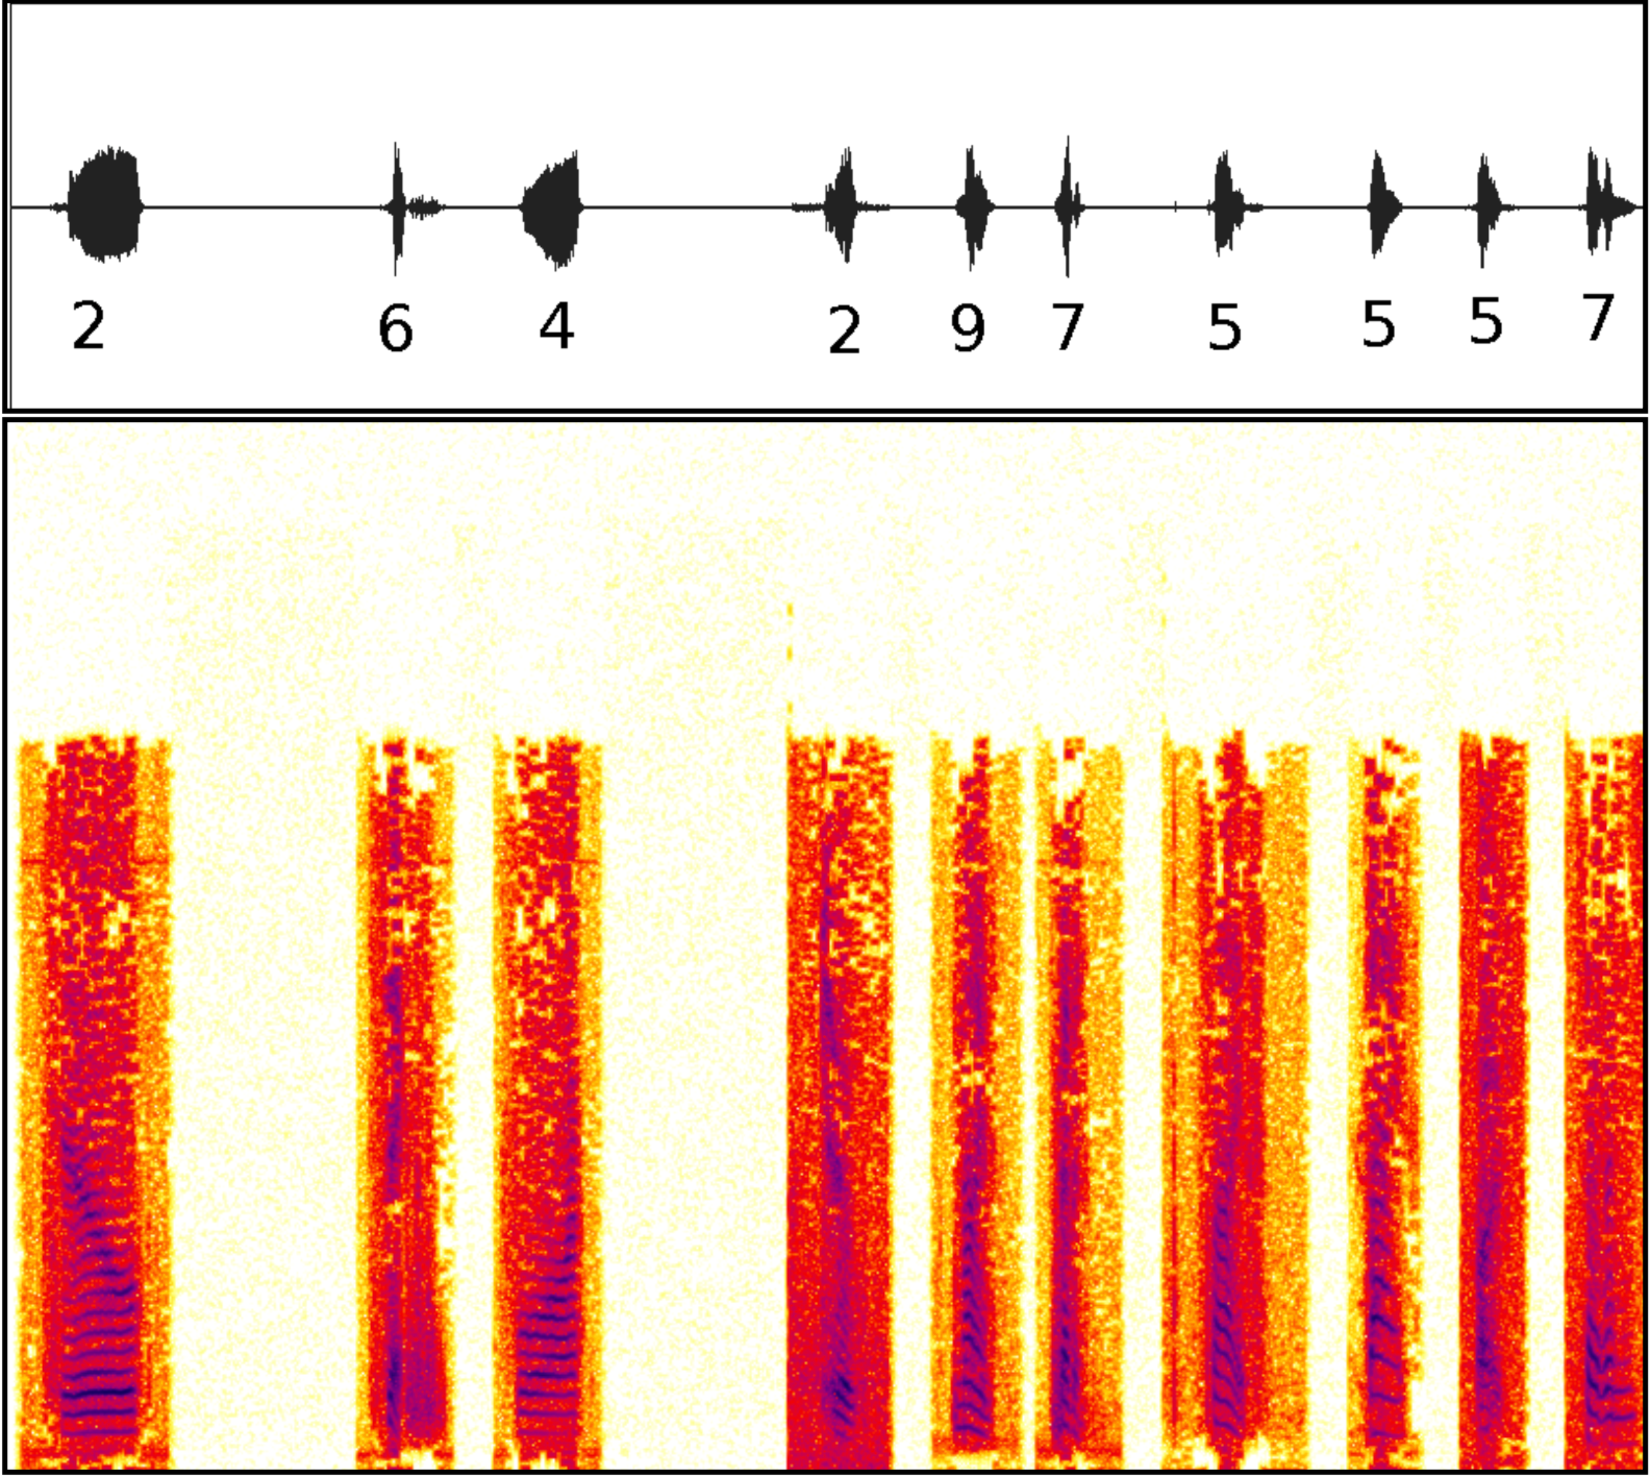
\includegraphics[width=\textwidth]{figures/recaptcha1.pdf}
        \caption{\re v1}
        \label{fig:recaptcha1}
\end{subfigure} \hspace{0.03\textwidth}
\begin{subfigure}{0.3\textwidth}
        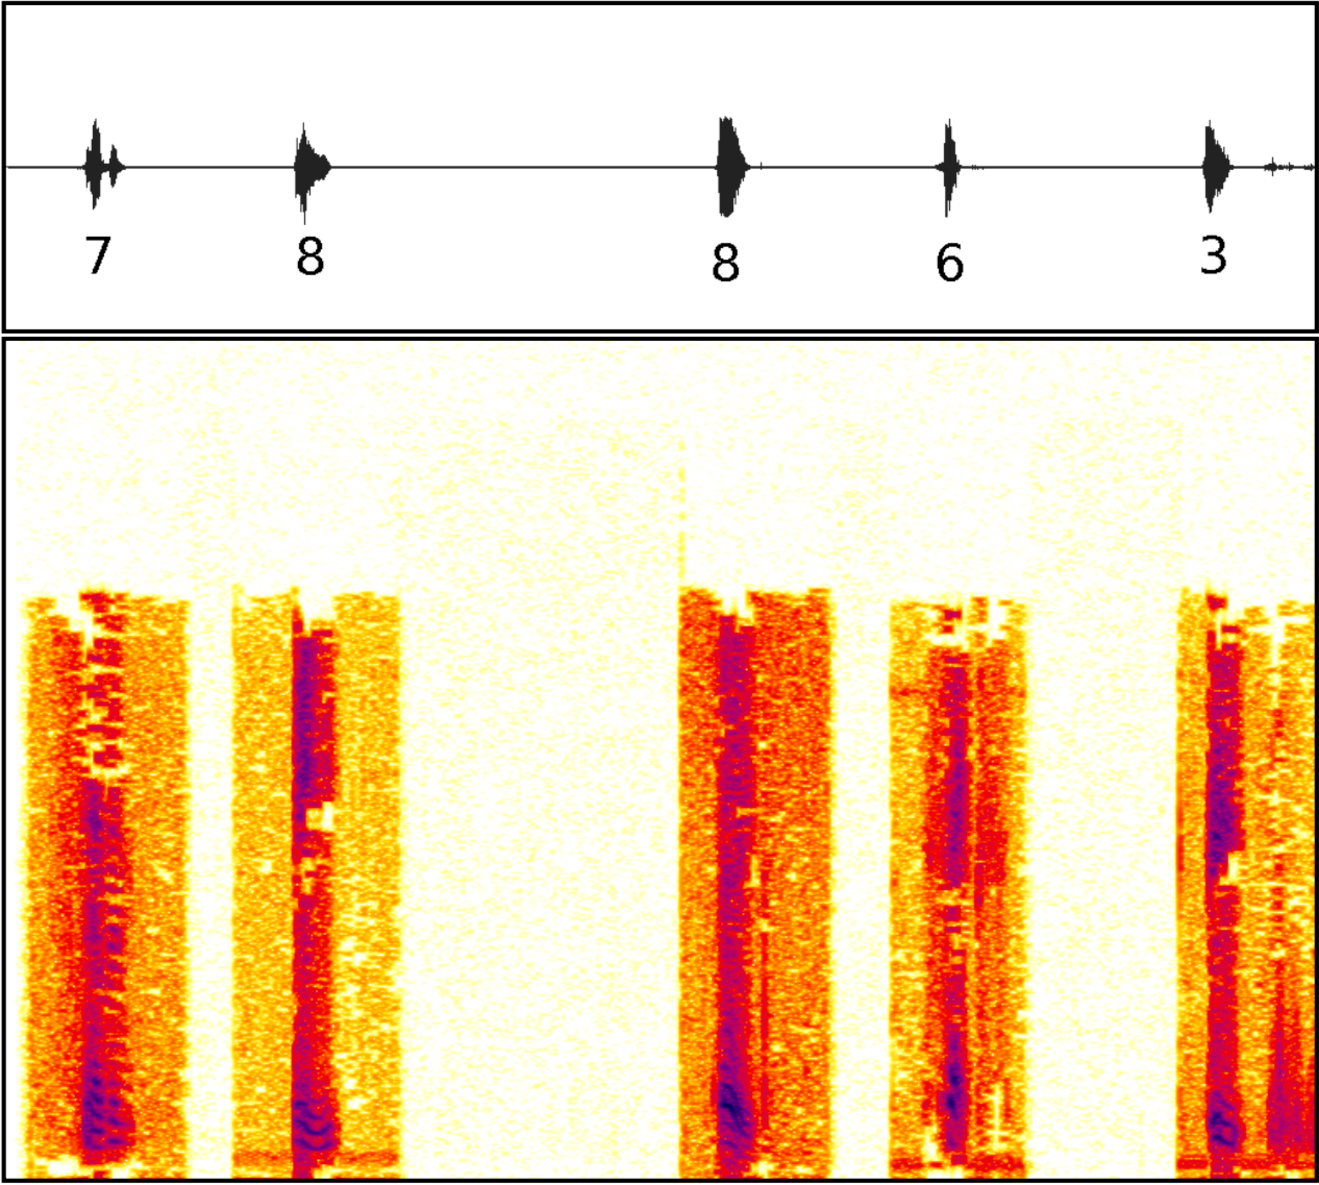
\includegraphics[width=\textwidth]{figures/recaptcha2a.pdf}
        \caption{\re v2.a}
        \label{fig:recaptcha2a}
\end{subfigure}\hspace{0.03\textwidth}
\begin{subfigure}{0.3\textwidth}
        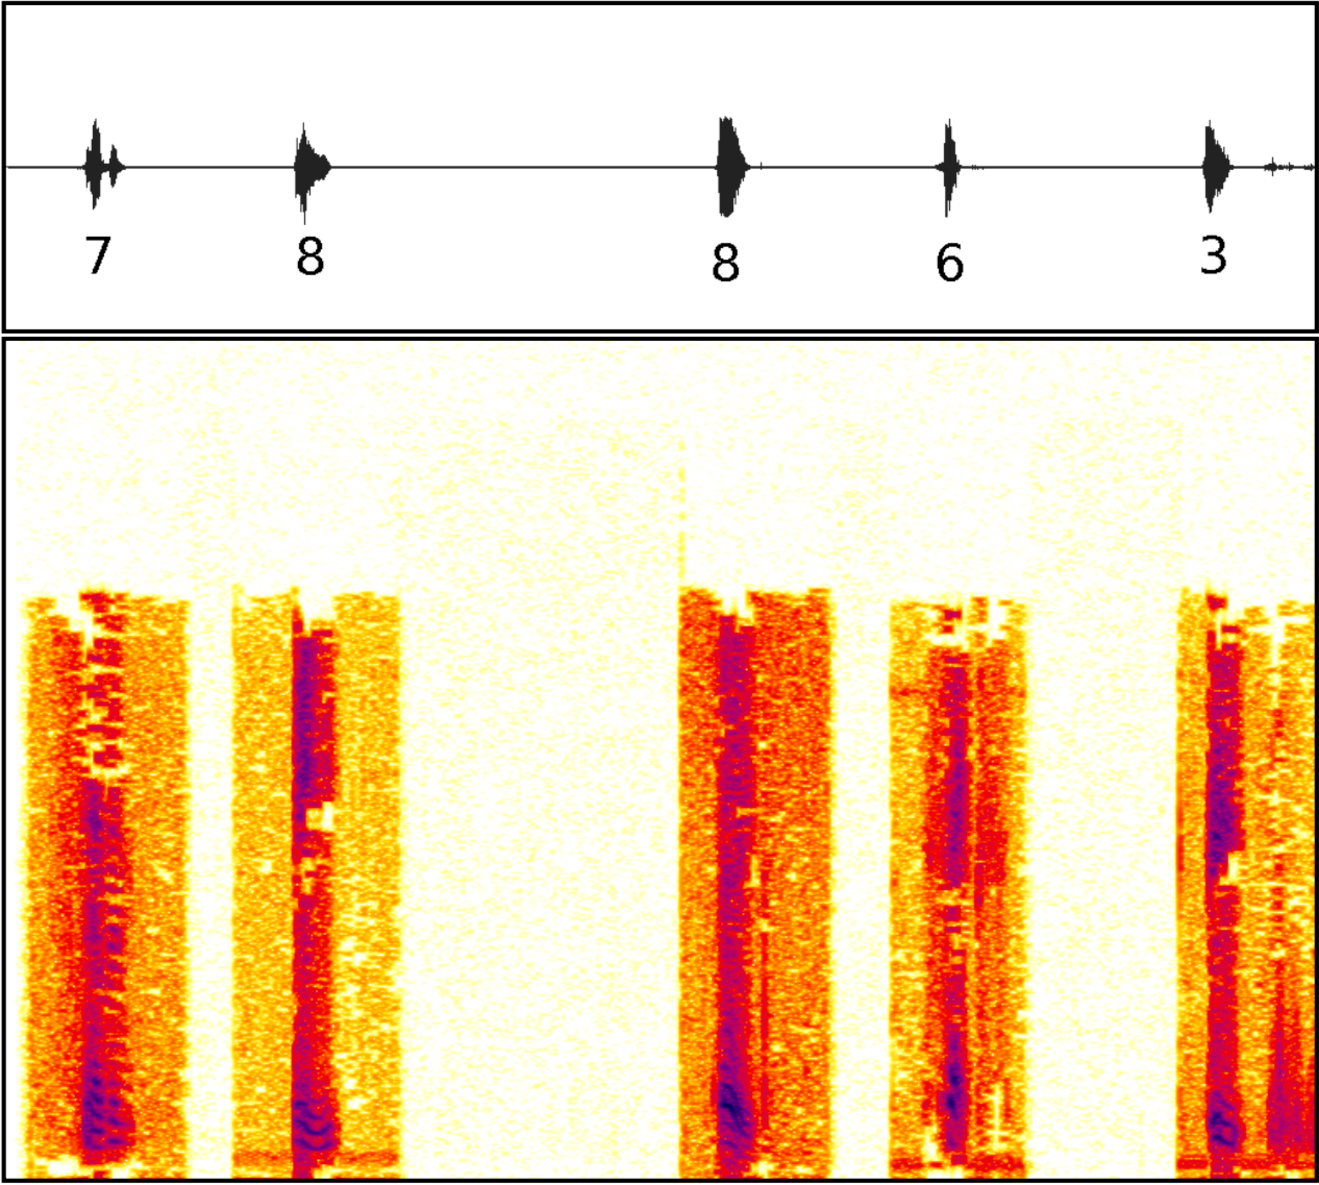
\includegraphics[width=\textwidth]{figures/recaptcha2a.pdf}
        \caption{\re v2.b}
        \label{fig:recaptcha2b}
\end{subfigure}
\caption{Waveforms and corresponding spectrograms for a sample audio challenge from the different versions of Google \re.}
\label{fig:examples}
\end{figure*}

Google's Recaptcha system is the most widely deployed captcha system, which is continuously tweaked to 
adapt to publicized attacks. During our experiments there was a significant change in the audio challenges,
and we will differentiate between the 2 versions in the remainder of the paper.

%Google provides a demo page for Recaptcha, its state-of-the-art captcha system (the version 2 of Recaptcha), 
%accessible via the following URL (https://www.google.com/\newline recaptcha/api2/demo), for anyone who wants 
%to try out the new captcha system. We used this demo page for all our tests on Recaptcha. The page connects 
%over HTTPS and does not require a login. The page initially loads a widget with a checkbox, which on clicking, 
%shows another widget with the image captcha that loads in a new iframe. The audio captcha challenge appears only 
%after clicking on the headphones-like icon in the bottom of the second widget.

\textbf{Recaptcha 2a.}
The audio challenge provided by the recaptcha system spells out 5 digits (the system has now been updated with 
10 digits) consecutively with little or noise, which the user must then identify and enter into the textbox provided. 
The interval between the digits is not a constant value. Each digit may be spelled out by the same person or different 
persons, male or female. Accents do not generally differ to a large extent.

The challenge also provides an option for the user to download the .mp3 version of the audio. The recaptcha system provides 
a margin for error and allows up to 2 incorrect digits out of the 5. We demonstrate how this high margin for error can be 
leveraged to get an almost 100\% accuracy value. We were able to exploit a security flaw in this system that allowed us to 
bypass the rate limiting that was in place.

The recaptcha demo page generates a new captcha challenge each time we connect to it. It behaves exactly like the recaptcha 
v2 widget that is embedded in popular websites such as Quora, BusinessInsider, Twitter, Ticketmaster and many more, as part 
of their account creation process. This was one of the main reasons why we chose to do our tests with the demo page, instead 
of any particular website that employs Google's recaptcha. Our results would thus stay valid on any website that has the latest 
recaptcha widget embedded.

\textbf{Recaptcha 2b.} The latest version of Recaptcha (as of early 2017) is known as the invisible Recaptcha 
(accessible via the following URL https://www.google.com/recaptcha/api2/\newline demo?invisible=true). This 
version does not have an explicit checkbox as seen in the previous version. It relies heavily on the number 
of requests generated per IP address, cookies and other parameters rather than the text/audio challenge itself. 
If the system does not suspect bot activity, it automatically authenticates the user as real even without presenting 
the user with a challenge (i.e. without any user interaction). However, a challenge is presented when the system 
suspects bot activity, and this challenge is very similar to the previous version with respect to the look and feel.

When accessed from a private browsing session, as there are no cookies, the system is suspicious and requires a challenge 
to be solved. This version spells out 10 digits in its audio challenge consecutively with little or no noise at all, with 
an error margin of 1 digit and also allows downloading of the MP3 file from the interface itself. Although we were very 
easily able to transcribe the digits of the audio, we were unable to bypass the rate-limiting that has been set by the system.

\textbf{Recaptcha 1.0} Although still used in many websites, Google has discontinued this version of Recaptcha since 2014. 
Signing up for Recaptcha now enables the newer version by default. It must be
noted that the websites that used this version previously did not automatically upgrade to the No 
captcha Recaptcha version, and they remain open to the vulnerabilities that were fixed in the subsequent 
version. We have obtained \note{X} samples from the authors of prior work~\cite{meutzner2014using} so as to 
compare the effectiveness of our attack that users off-the-shelf speech recognition systems against previous 
studies that trained their own machine learning classifiers.

There are 10 digits that are spoken in the audio challenge and there is very little or no noise. This 
version does not enforce any rate limiting unlike the newer versions of Recaptcha. The margin for error 
is again 1 out of the 10 spoken digits. With respect to the text based challenge, there are two words 
shown which must be recognized by the user and typed into the input field. The first word is an unknown 
text from a failed OCR scan while digitizing physical books and other printed material, and the other 
being a ``control'' word, which is known. This helped transcribe the unknown words and digitize them, and 
in 2012, photographs of house numbers taken from Google's Street View project began to be used, in 
addition to scanned words. 

\begin{figure*}[tp]
\begin{subfigure}{0.3\textwidth}
        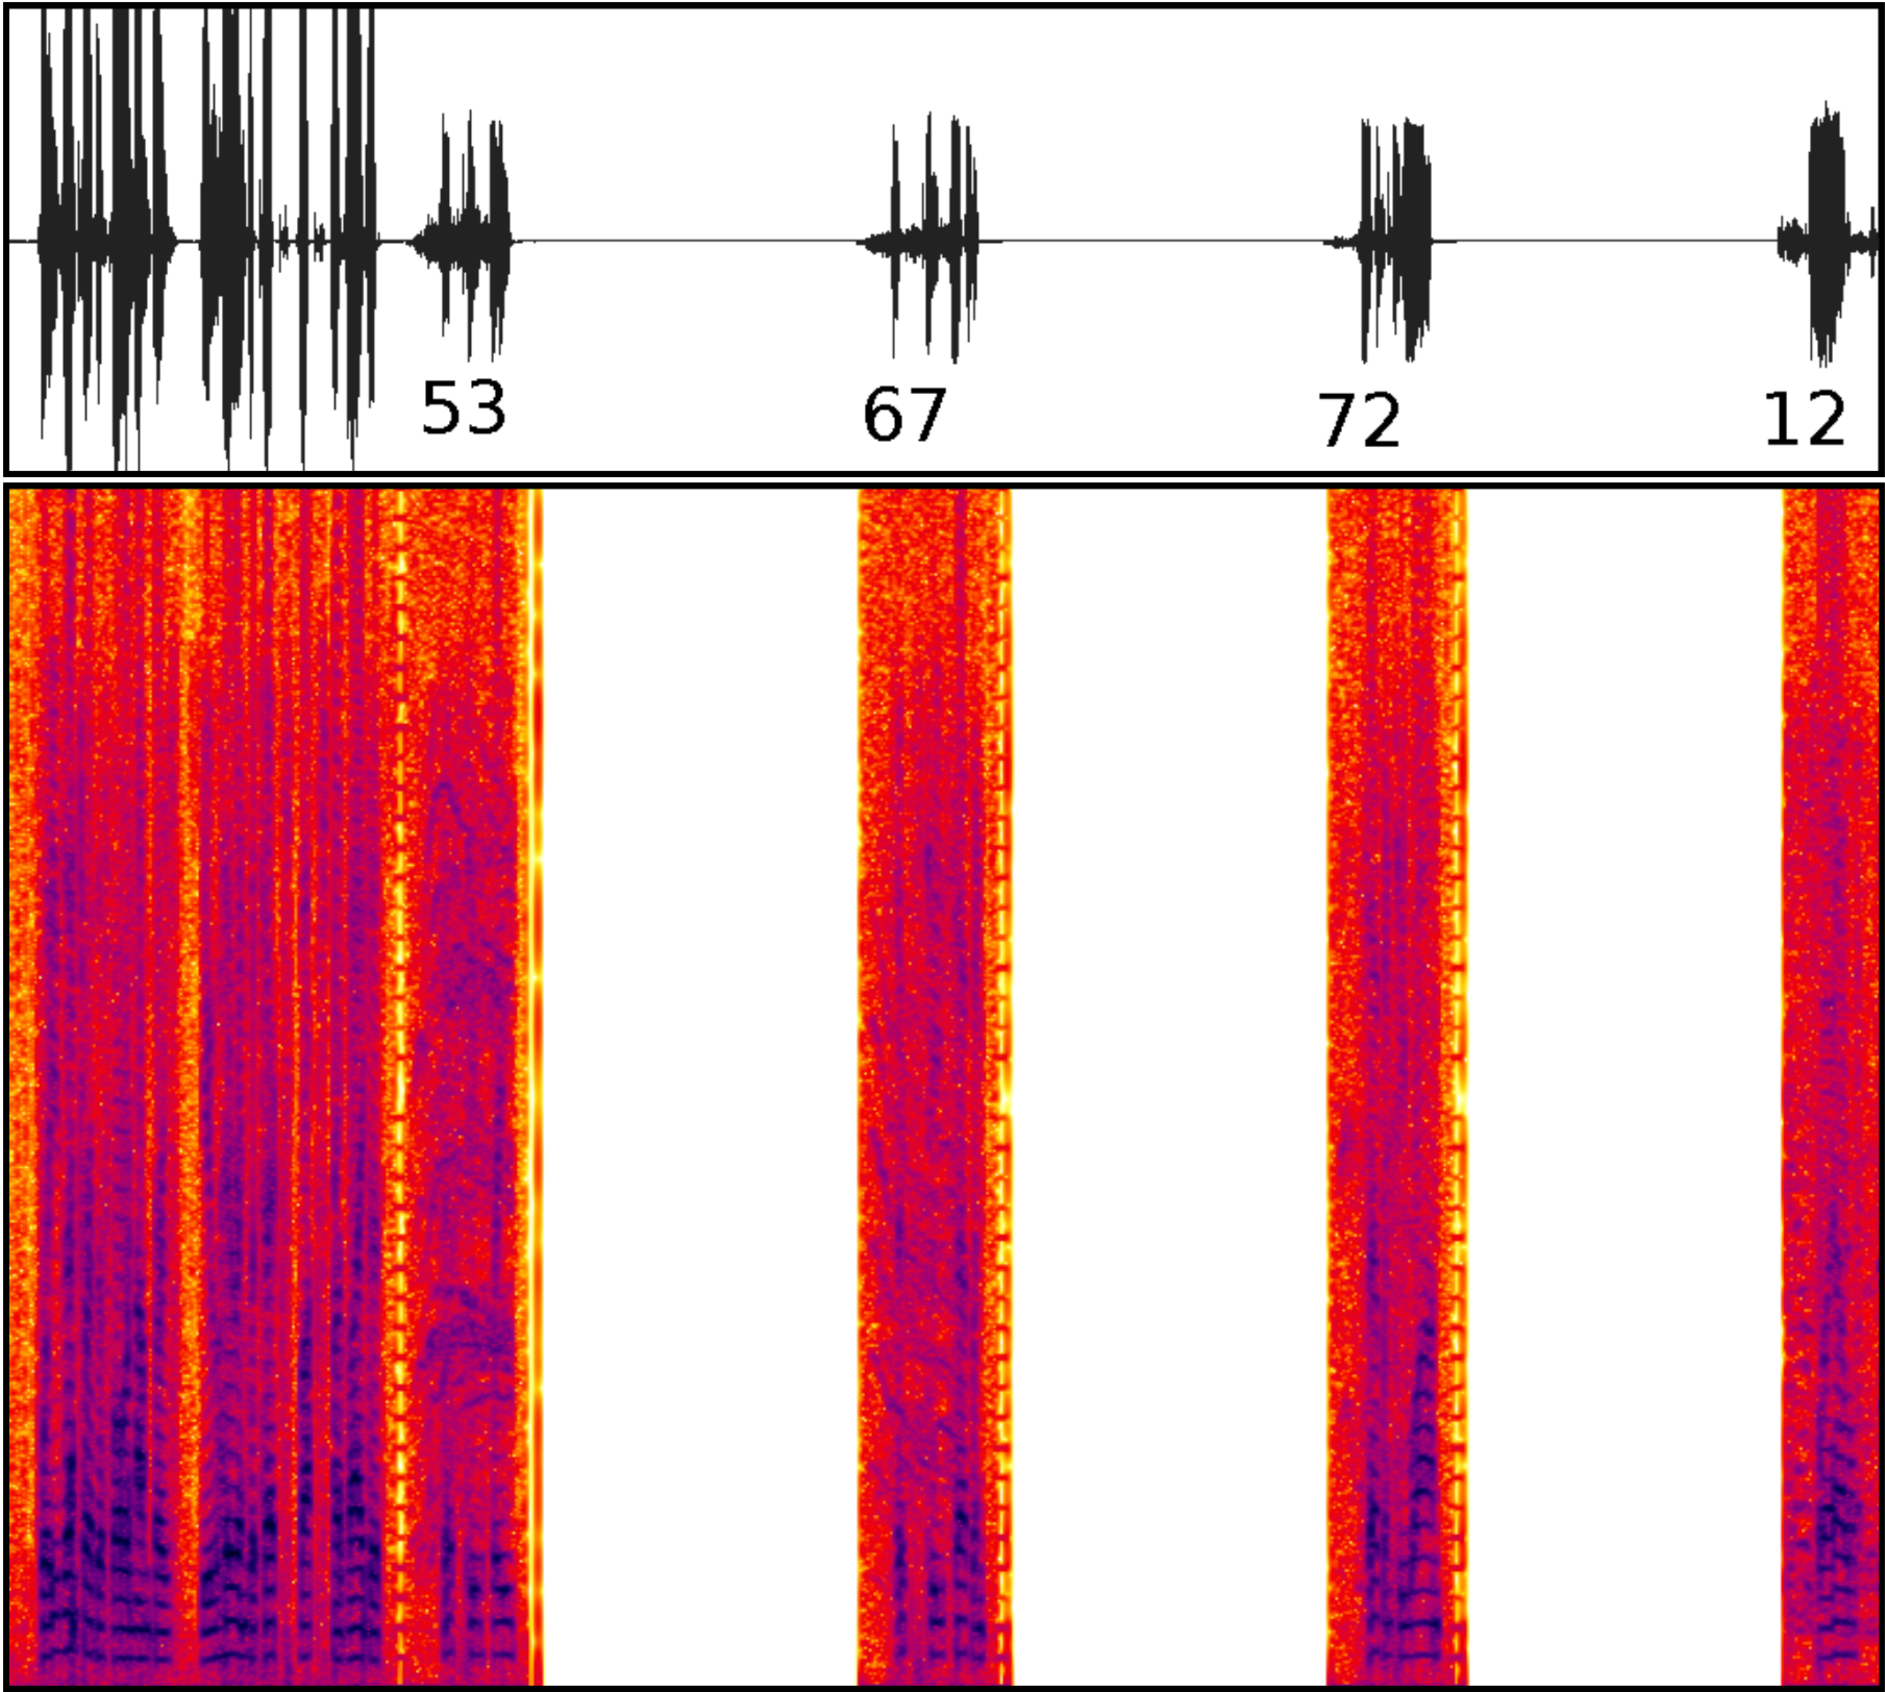
\includegraphics[width=\textwidth]{figures/apple.pdf}
        \caption{Apple}
        \label{fig:apple}
\end{subfigure} \hspace{0.03\textwidth}
\begin{subfigure}{0.3\textwidth}
        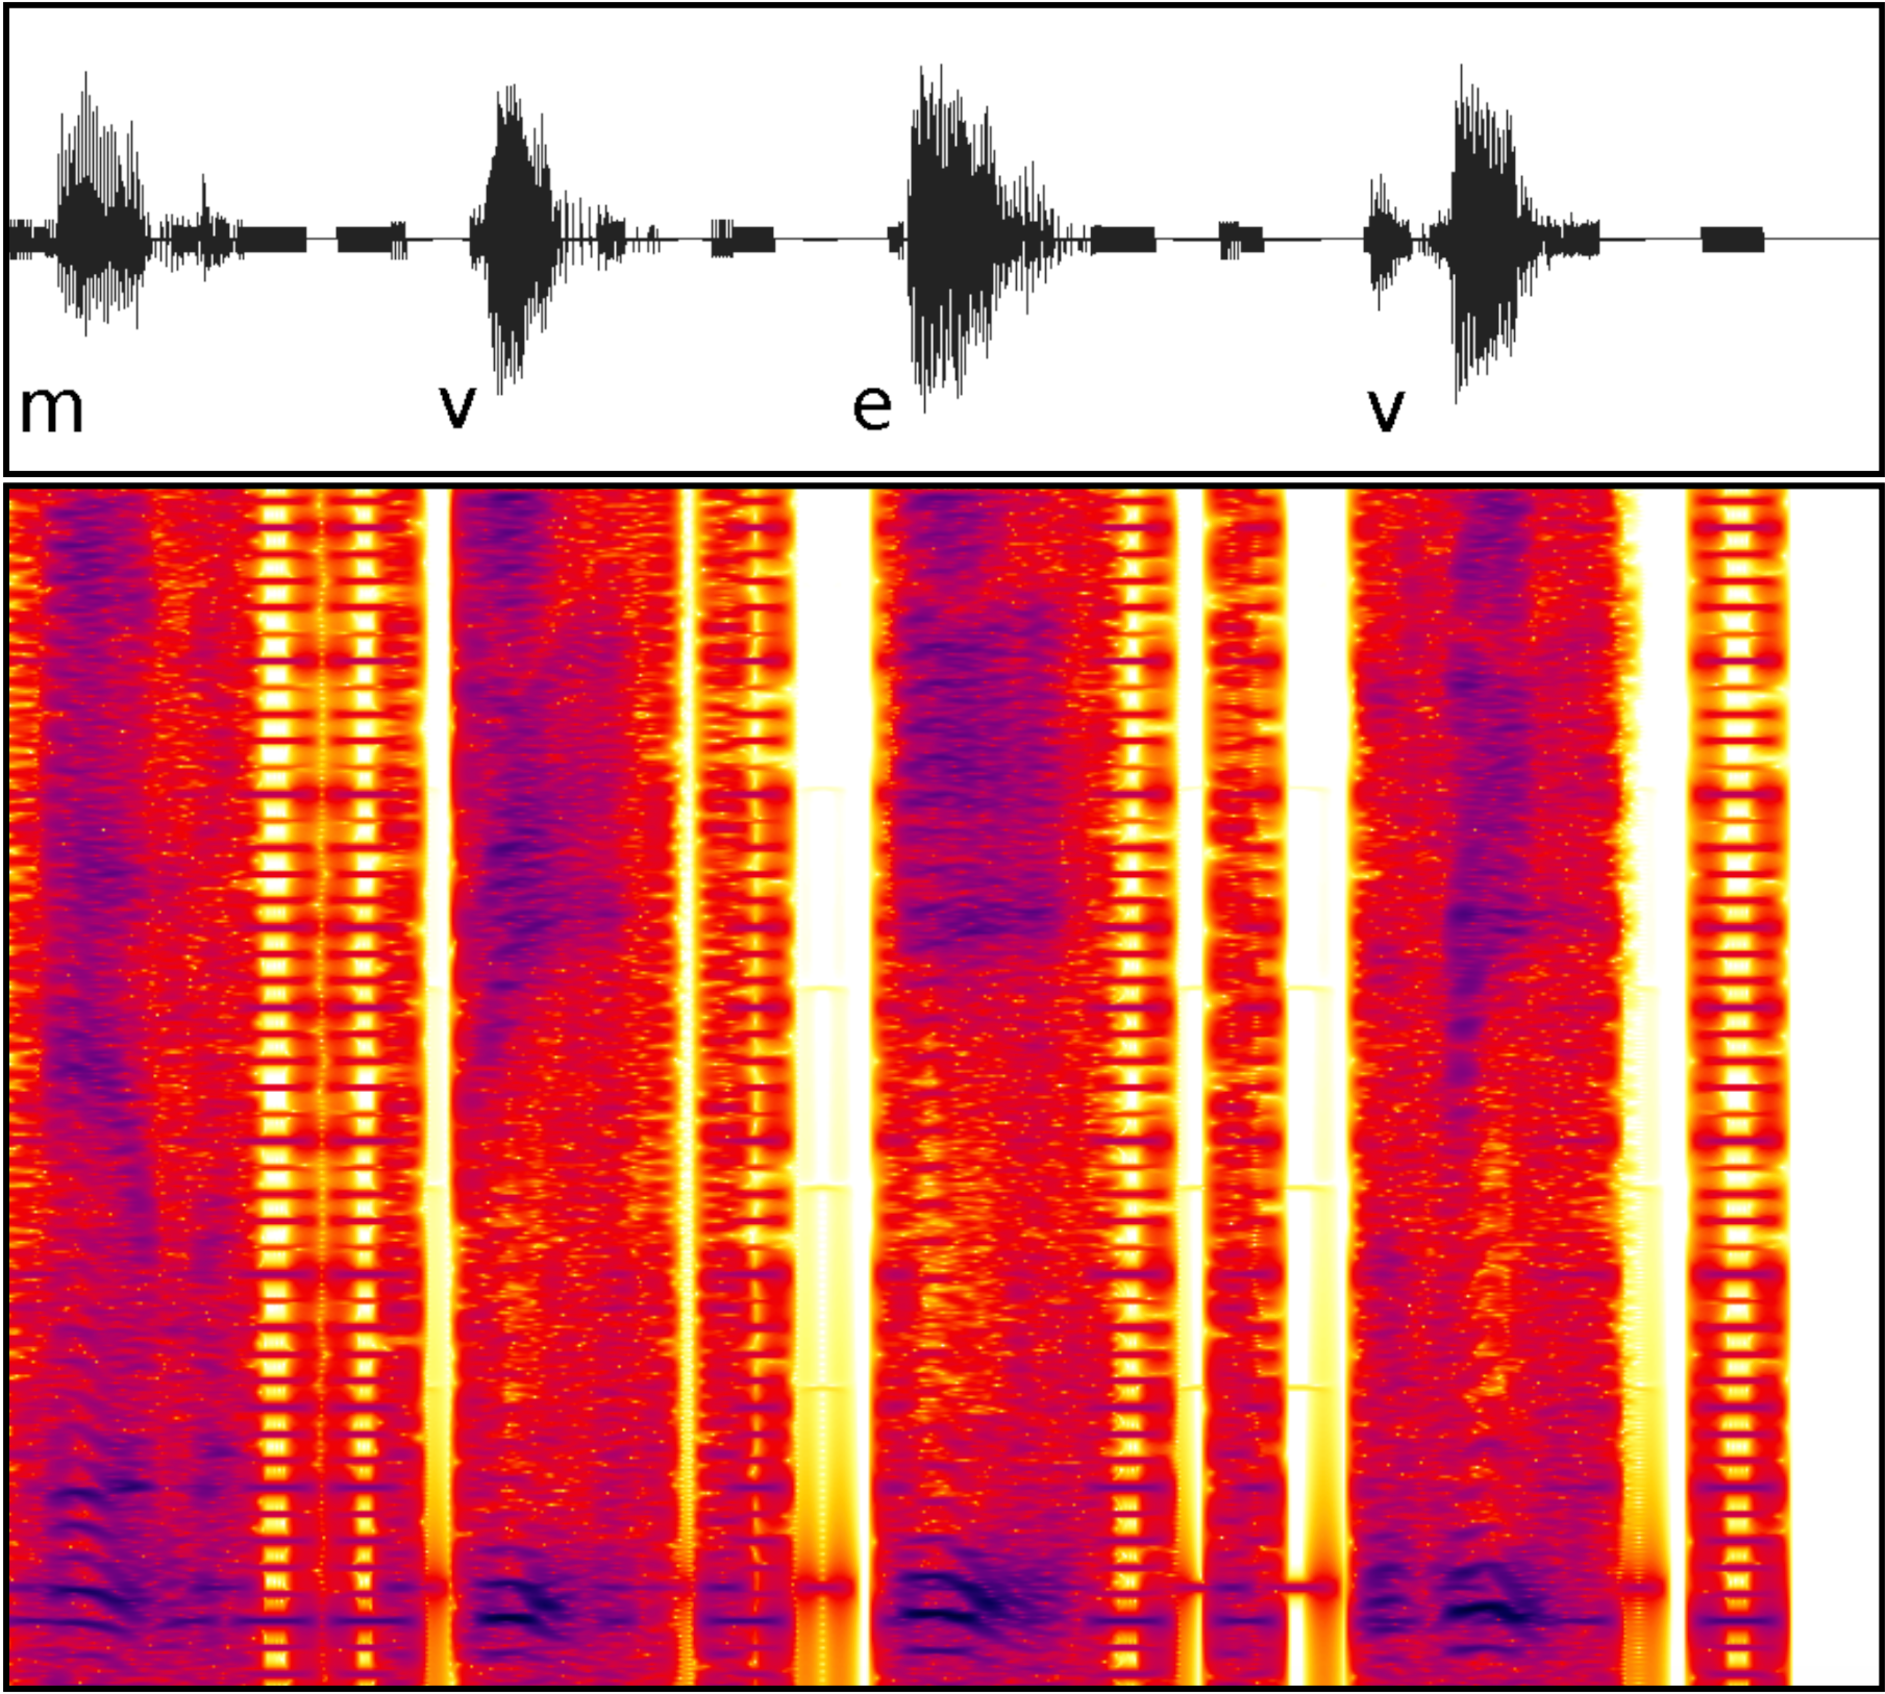
\includegraphics[width=\textwidth]{figures/botdetect.pdf}
        \caption{BotDetect}
        \label{fig:botdetect}
\end{subfigure}\hspace{0.03\textwidth}
\begin{subfigure}{0.3\textwidth}
        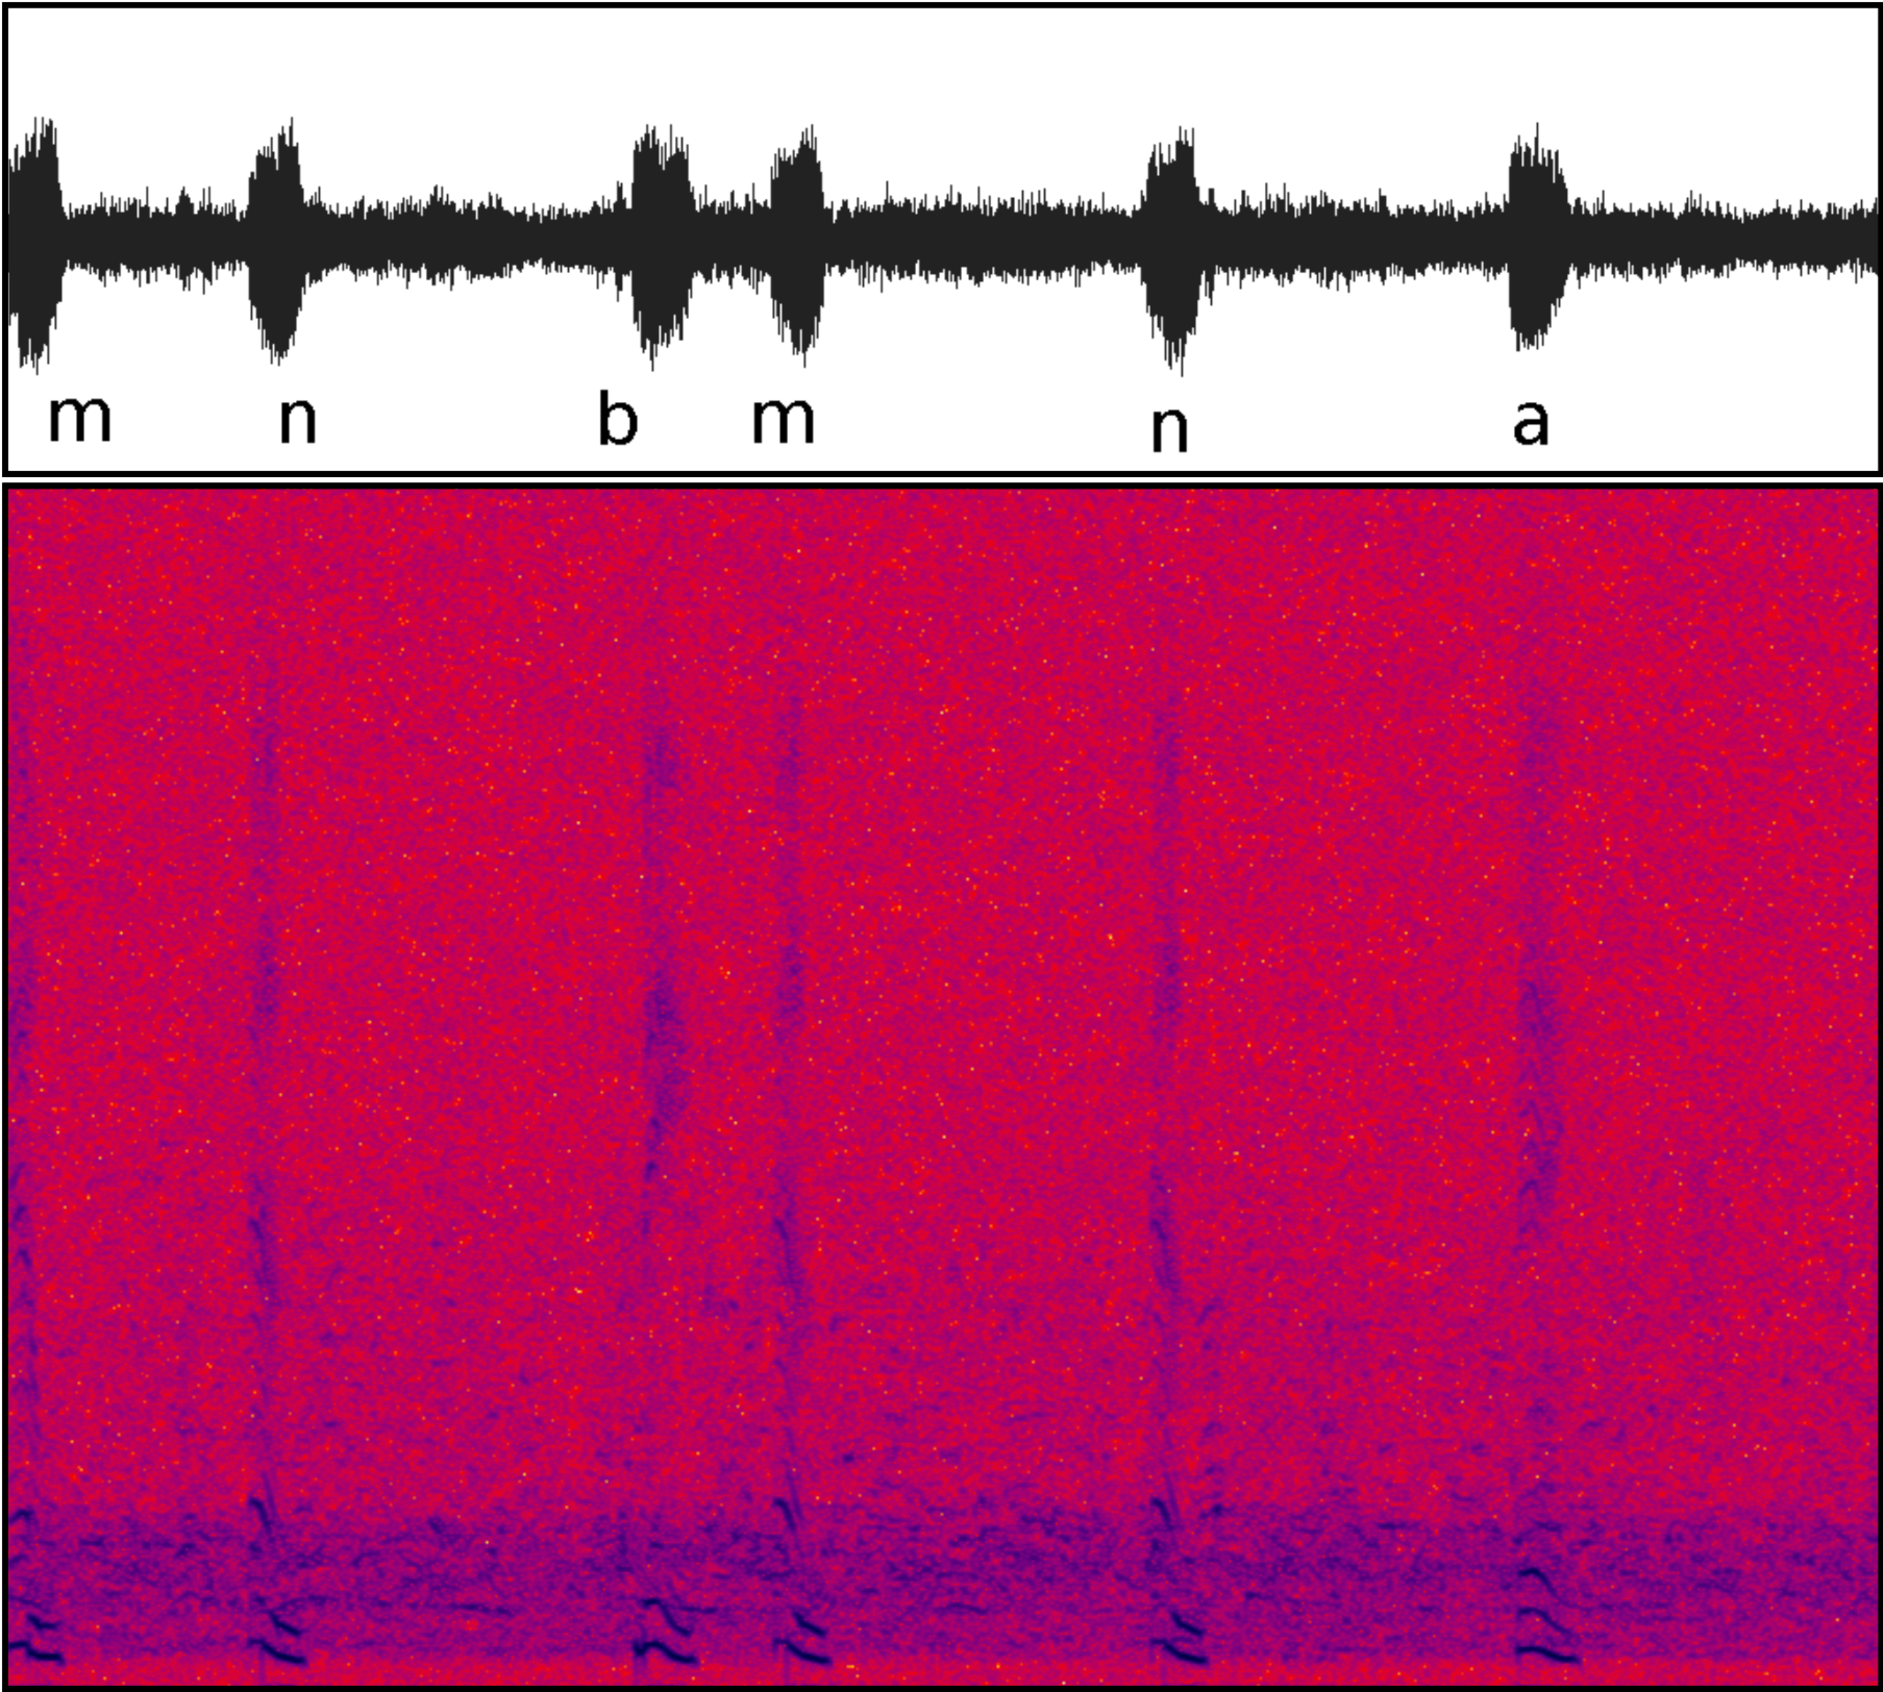
\includegraphics[width=\textwidth]{figures/captchas.pdf}
        \caption{Captchas.net}
        \label{fig:captchas}
\end{subfigure} \\
\begin{subfigure}{0.3\textwidth}
        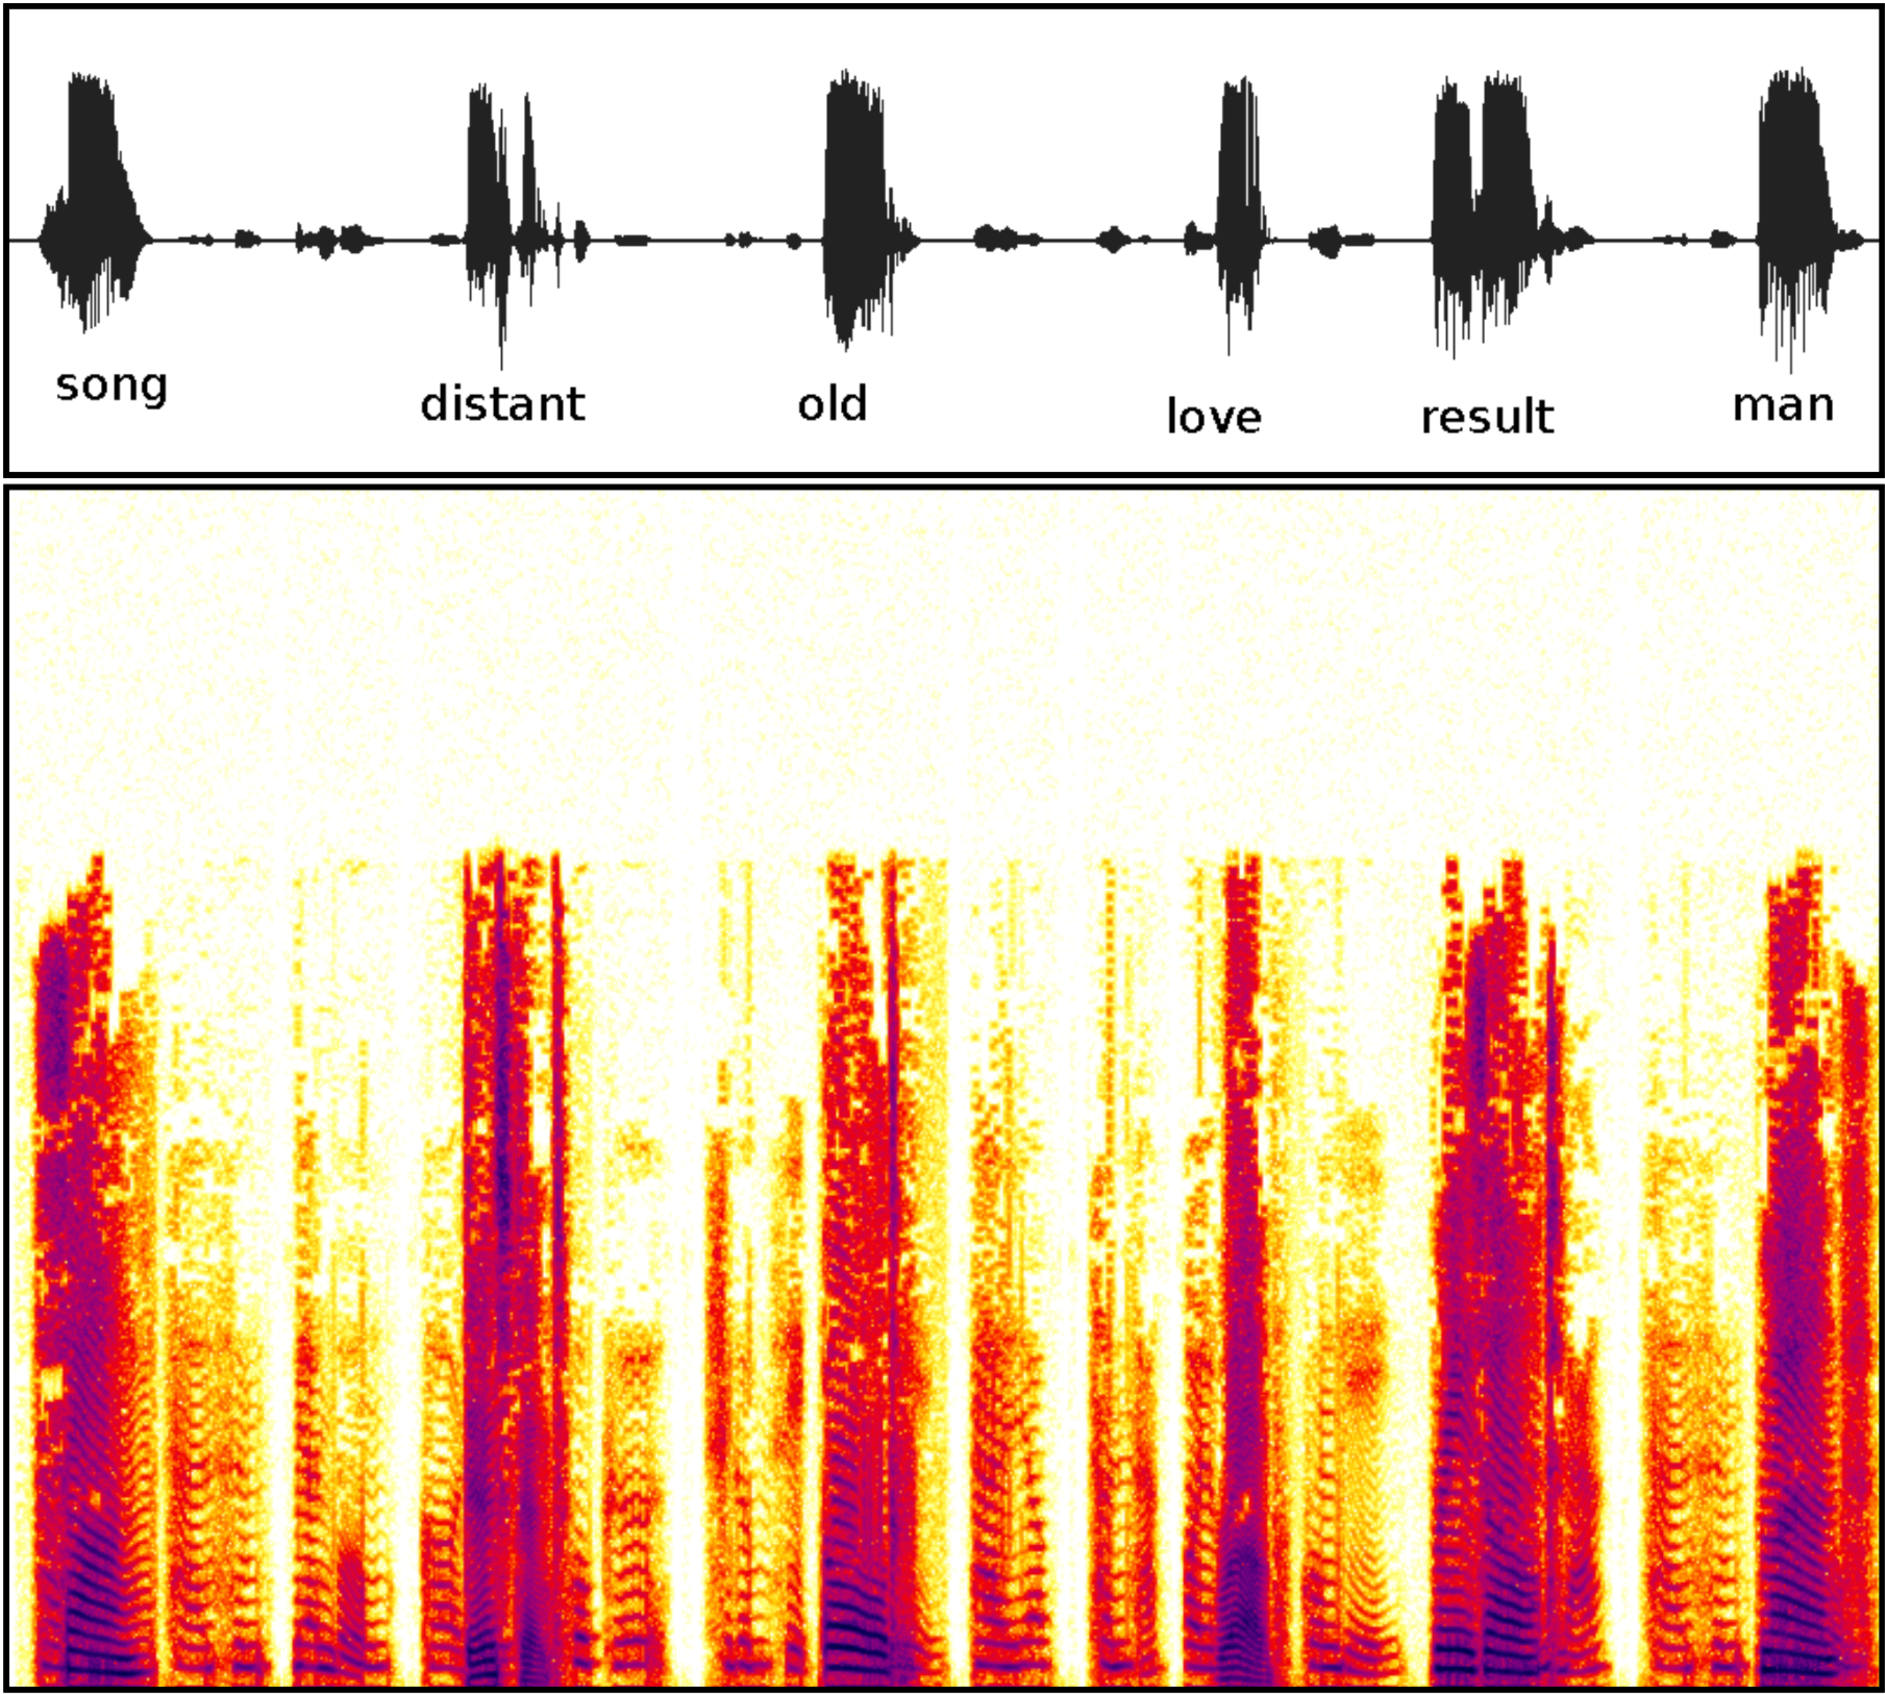
\includegraphics[width=\textwidth]{figures/live.pdf}
        \caption{Microsoft}
        \label{fig:live}
\end{subfigure}\hspace{0.03\textwidth} 
\begin{subfigure}{0.3\textwidth}
        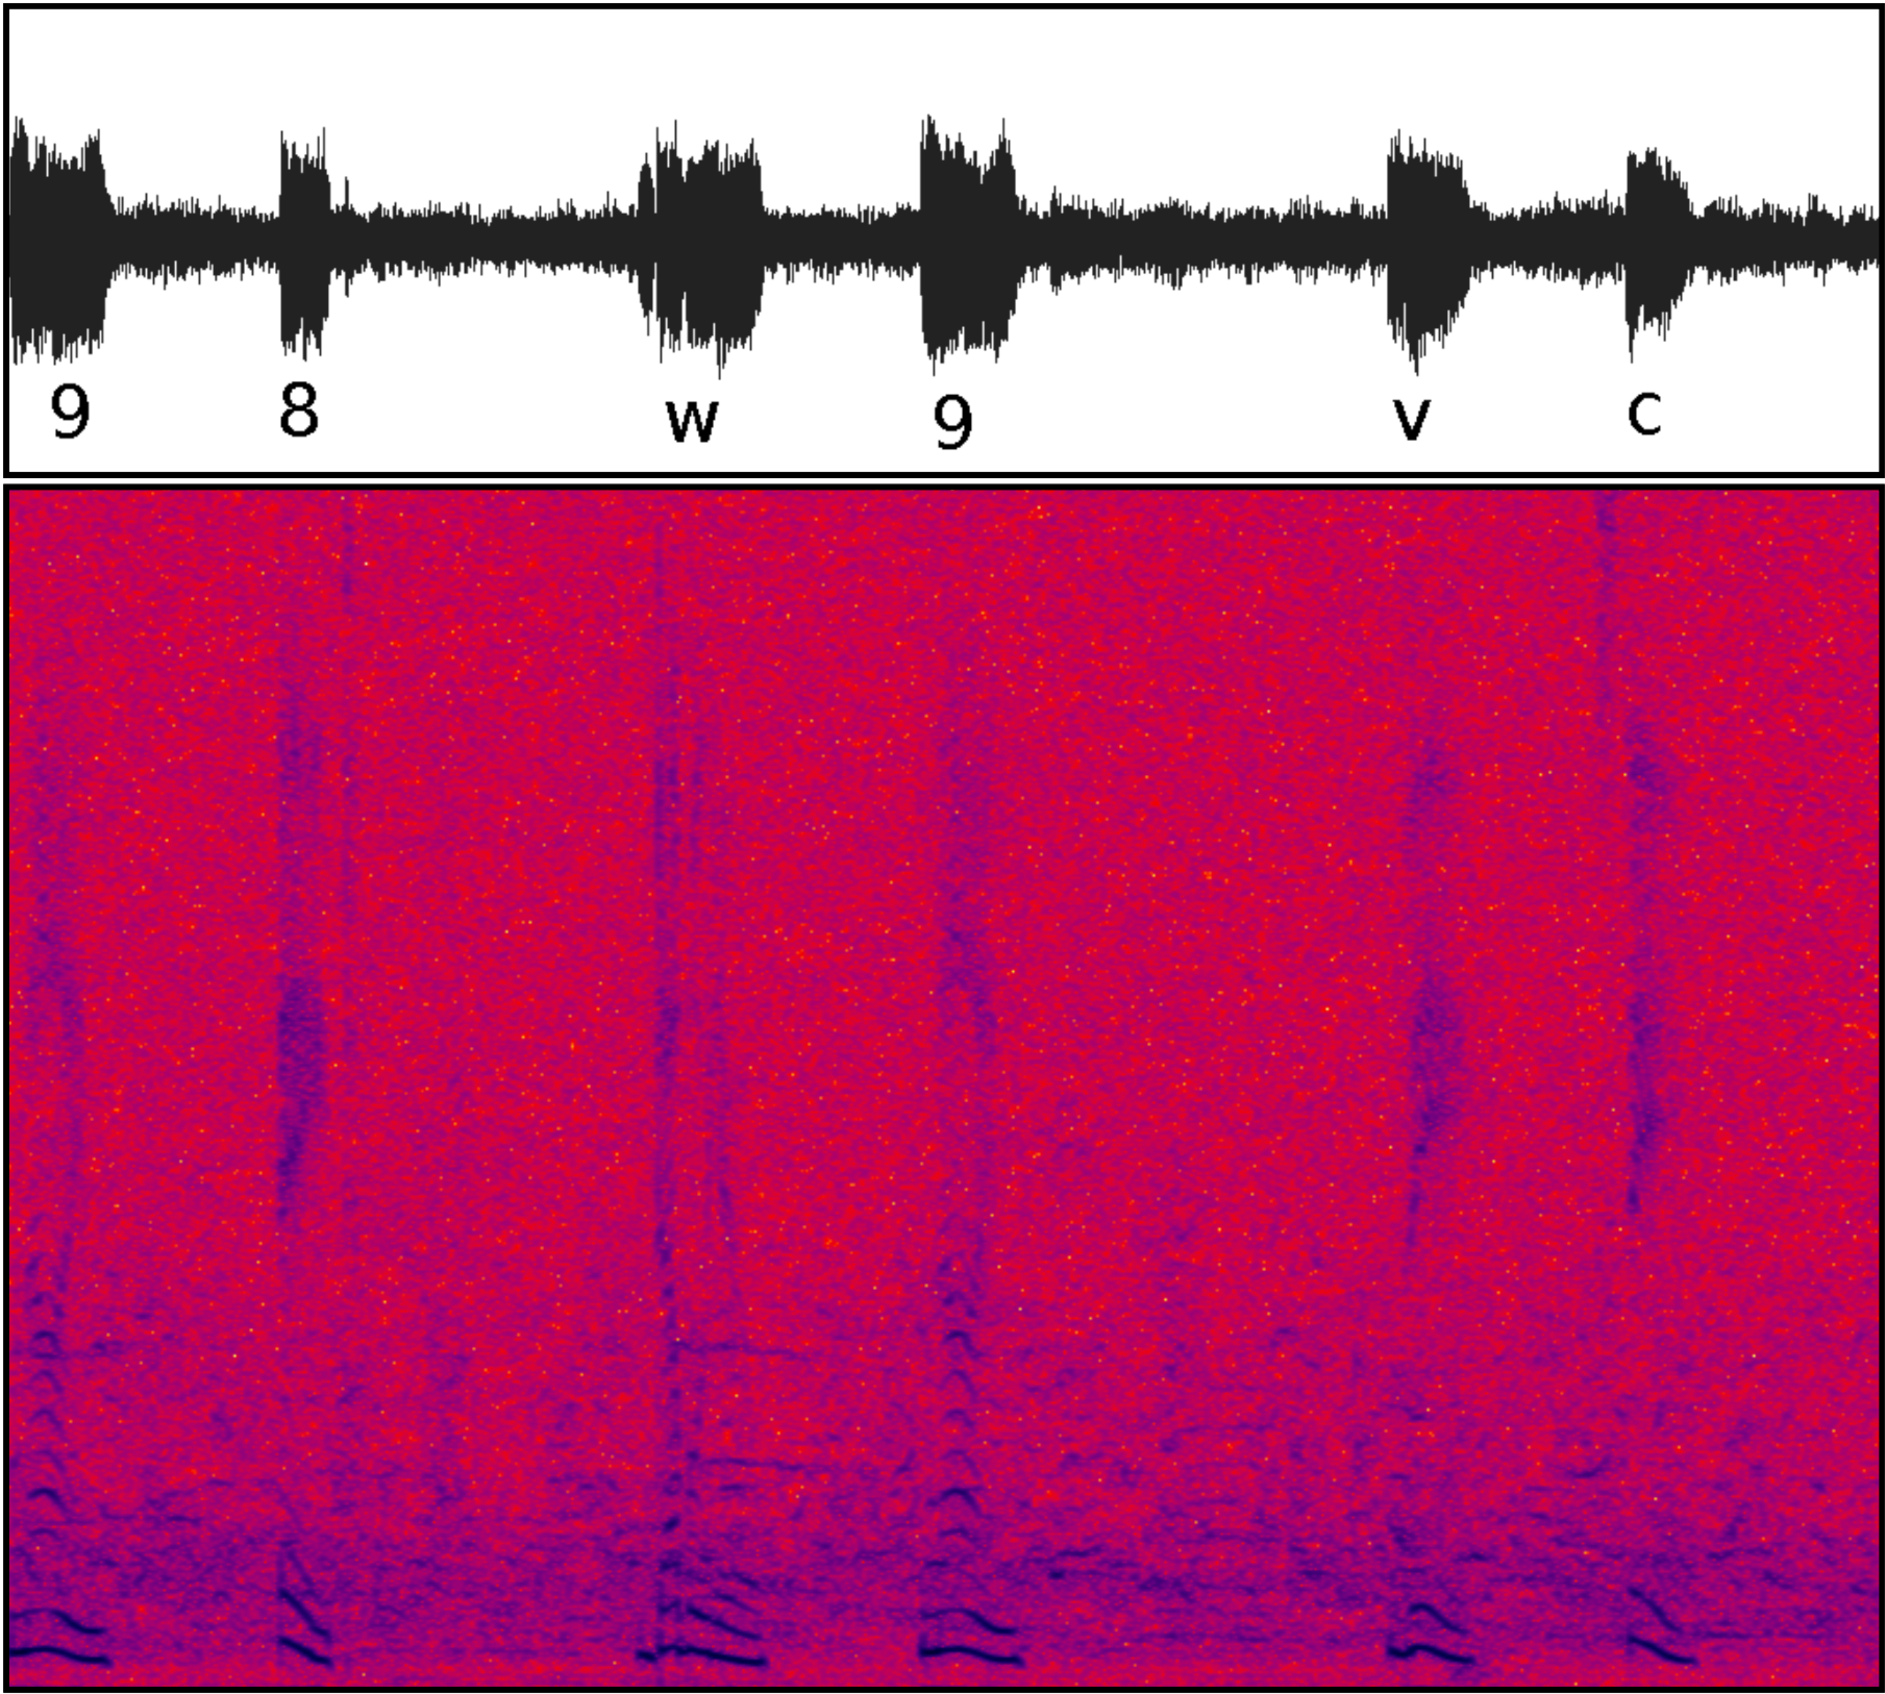
\includegraphics[width=\textwidth]{figures/secure.pdf}
        \caption{SecurImage}
        \label{fig:secure}
\end{subfigure}\hspace{0.03\textwidth}
\begin{subfigure}{0.3\textwidth}
        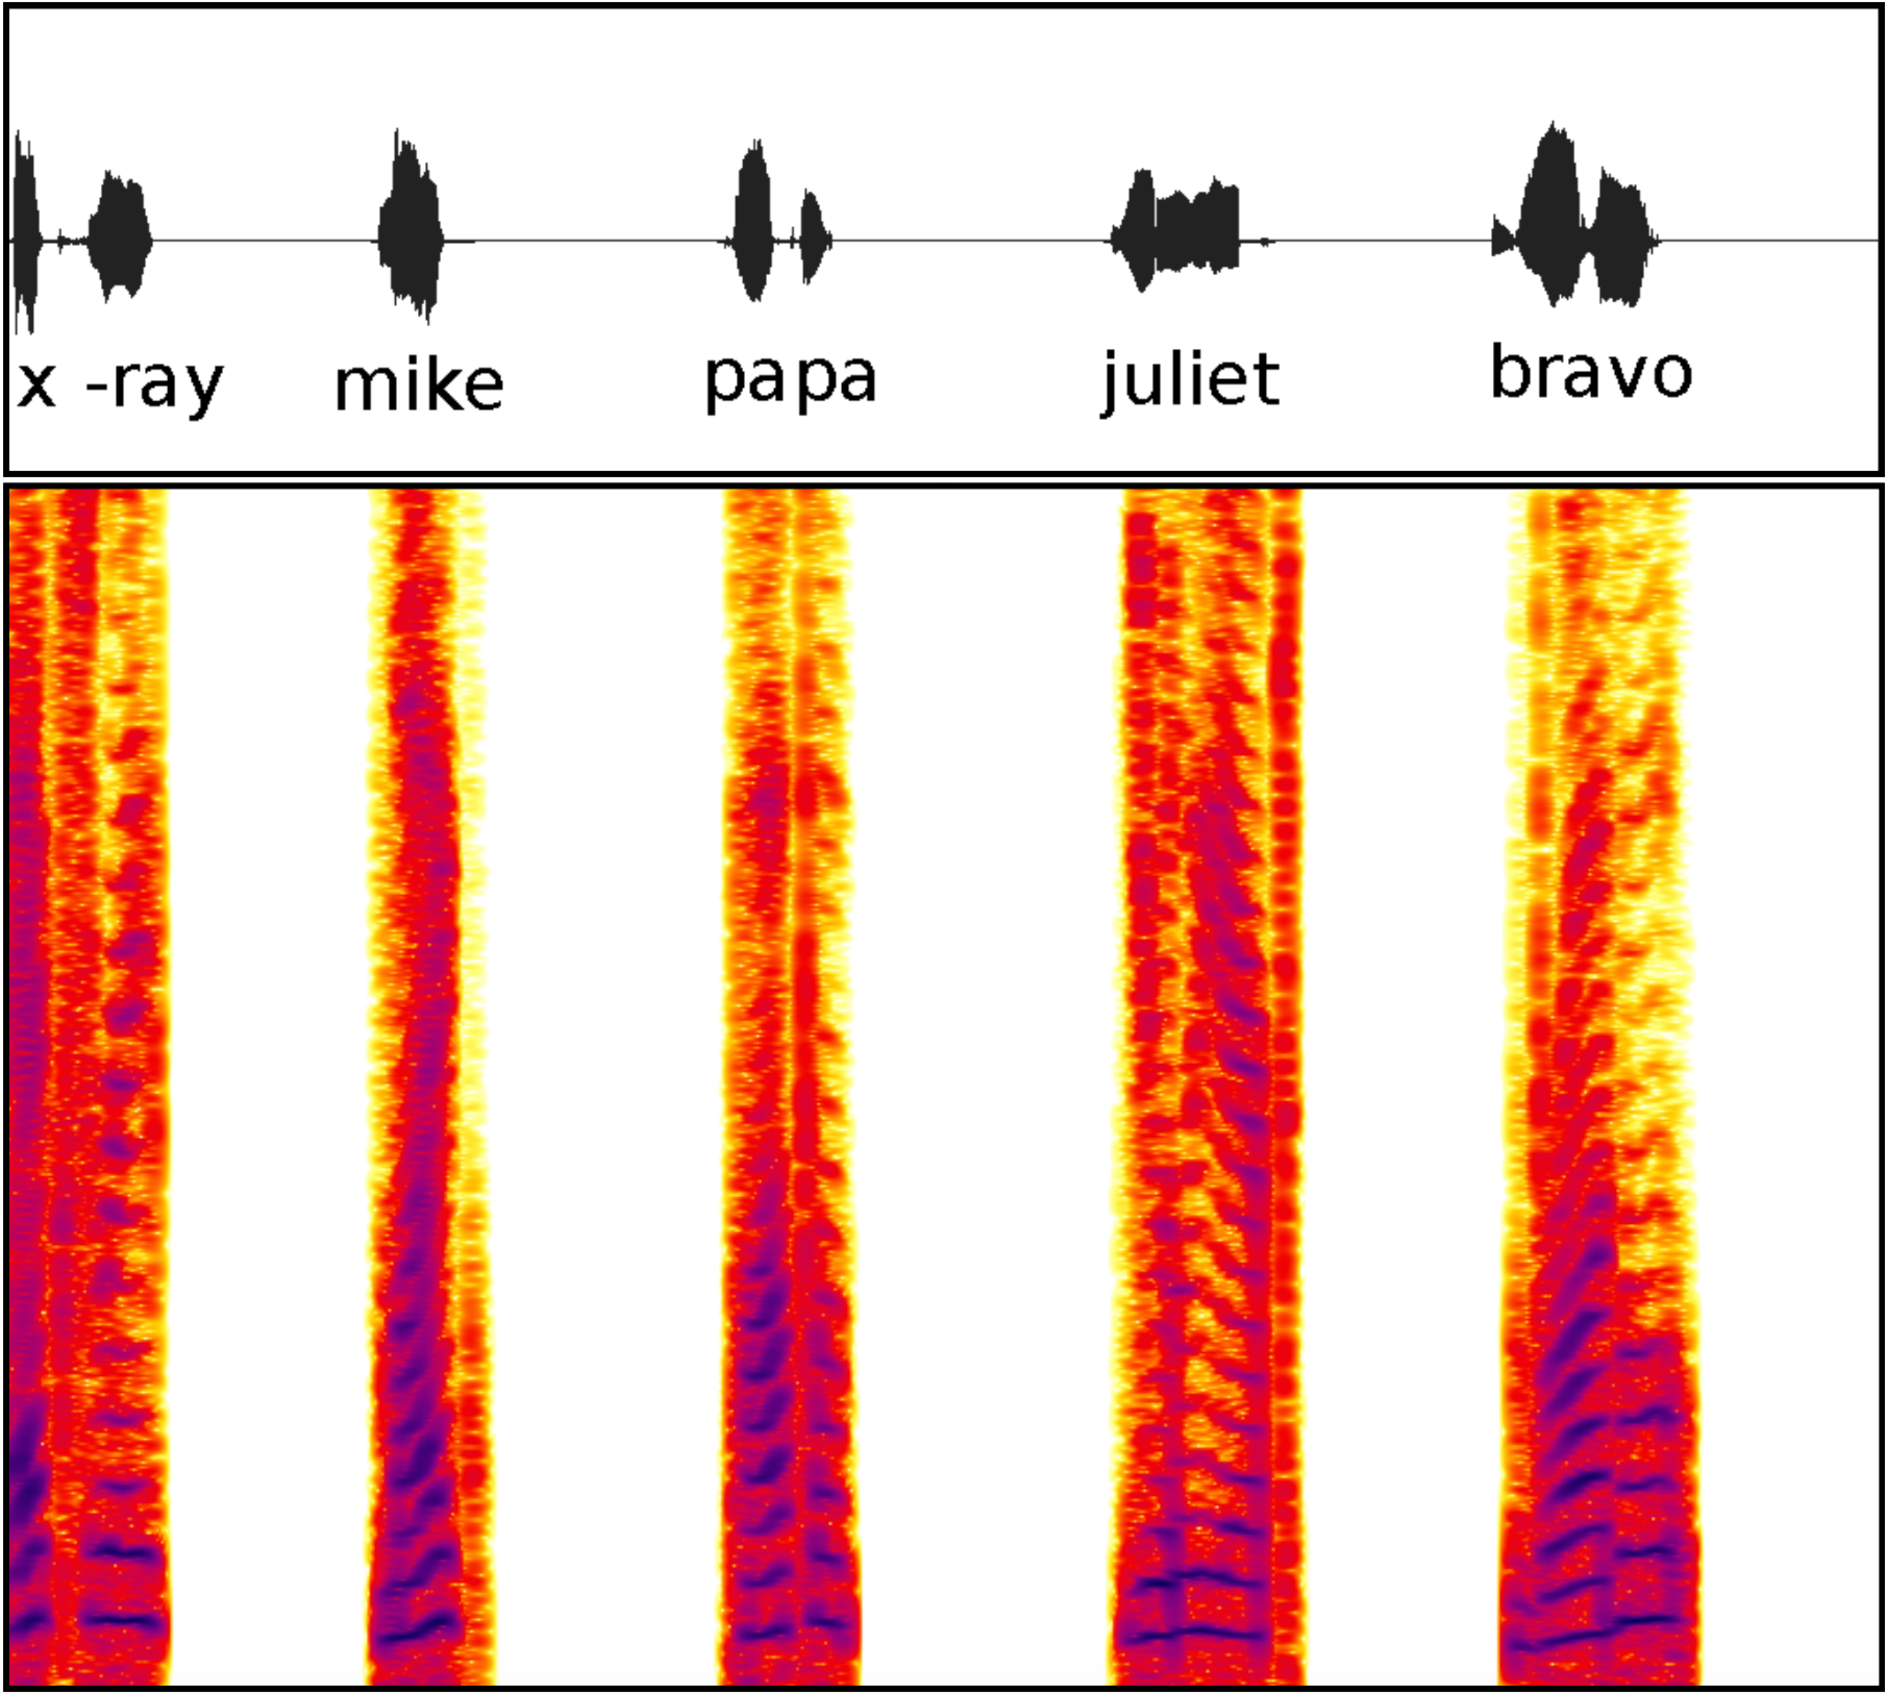
\includegraphics[width=\textwidth]{figures/telerik.pdf}
        \caption{Telerik}
        \label{fig:telerik}
\end{subfigure}
\caption{Waveforms and corresponding spectrograms for a sample audio challenge from every captcha service.}
\label{fig:examples}
\end{figure*}

\subsection{Securimage}

Securimage is an open source captcha system that was developed by Drew Phillips that has 
been under active development and maintenance since 2005. It also has plugins/modules for 
major content management systems like Drupal, Wordpress, Joomla!, etc. It is written in PHP 
and offers very easy integration with websites written in PHP with a lot of customization 
options for both image and audio based challenges. The demo page contains 3 different forms 
of challenges - a random digit/character combination, a math puzzle and a custom captcha 
made from a word list. The demo page can be found here: https://www.phpcaptcha.org/
try-securimage/.

For each audio challenge, the system generates a WAV file from a corpus of audio files of 26 
alphabets (A-Z) and 10 digits (0-9). The digits and alphabets are spoken by only one person. 
The audio is generated by picking 6 word/digit files at random, combining them and adding one 
of the 5 noise files. The default number of digits/characters per challenge is 6, but this can 
be customized while implementing the library. Some other customization options are that one can 
specify a word list for the challenges and using a read-aloud math puzzle that is to be solved 
by the user. Securimage does not offer any margin for error.

\subsection{Captchas.net}

Captchas.net, started back in 2004 offers implementation and easy integration for PHP, ASP, Perl, 
Python, JSP and Ruby. It is a free service, but shows a watermark on the images of the text challenges 
which can be removed by subscribing to the paid version. For both the text and the audio challenges, 
Captchas.net follows the following method to validate the response:

\begin{itemize}
\item Both the client server and Captchas.net's server share a common secret key.
\item The secret key and a random string sent by the client are used to generate the password.
\item The password is computed by Captchas.net's server to generate the image and by the client server to validate the user's input.
\end{itemize}

The text challenges always consist only of alphabets and the audio challenge uses NATO alphabets 
of the same text challenge. For instance, ``RIPAZH'' would be read out as 'Romeo, India, Papa, Alpha, 
Zulu, Hotel' and the user is expected to enter the first letter of each uttered word. There is no 
margin for error in this service and there is little background noise.

\subsection{Apple}

Apple's captcha is encountered while signing up for a new iCloud account 
Before spelling out the audio challenge, 
the voice first says ``Please enter the $n$ numbers that you hear in the textbox provided''. The 
spoken numbers consist of two digits like 25, 64, etc. and they are always spoken by a single person. 
The page times out after two minutes of inactivity and a pop up appears for confirmation if the user is 
still in the process of creating the account. Apple does not allow downloading the audio file and is 
loaded and played via JavaScript and not stored in any cache or temporary storage.

To obtain the audio file for the challenge, one has to manually open the URL chrome://media-internals 
on the Google Chrome browser. The Media Internals feature of Chrome displays three things \cite{media}:
\begin{itemize}
\item Everything it can dig up from the media stack about active media players. Includes buffered data, 
    video properties, measured times between events, and a log of events.
\item Status and volume of active audio streams. These are not yet associated with a particular tab.
\item Cache activity, including reads from and writes to the media cache.\newline
\end{itemize}

\subsection{RadCaptcha by Telerik}

RadCaptcha is a captcha service by Telerik that is built especially for ASP.NET 
web applications. RadCaptcha and 90+ other controls are part of UI for ASP.NET AJAX, 
a comprehensive toolset that take care of the common functionality of a ASP based 
CMS like Sitefinity \cite{radcaptcha}. It is also a part of a feedback form for the 
HR website of UIC, where we discovered this captcha. It can be seen here: https://www
.hr.uic.edu/cms/One.aspx?pageId=356957\newline

RadCaptcha's audio challenge speaks out digits (0-9) and alphabets in NATO form. It is 
spelt out by a single speaker and there is almost no background noise in the audio. The 
audio is not available to download explicitly, but is present on the DOM of the web page 
in an <audio> tag, from which the URL of the audio file can be easily grabbed. One of the 
customizations provided by the service is a rate limit system, which requires the form to 
be displayed to the user for a particular number of seconds before it can be considered as 
human-submitted. However, this setting is left to the person who implements the captcha 
service on the web page.

\subsection{BotDetect}

BotDetect offers free and paid versions of its captcha system. In the free version, the 
service has several limitations, like the audio challenge is not fully functional most of 
the times. There is a 50\% chance that the audio challenge is replaced with an audio file 
that speaks "Sound Demo". BotDetect offers libraries for integration with .NET, Java, ASP 
and PHP based websites. The demo page of BotDetect can be accessed here: 
\url{https://captcha.com/demos/features/captcha-demo.aspx}.

The audio challenge speaks out exactly the digits and characters in the text/image challenge. 
While implementing the captcha service on one's website, the web master has a lot of customization 
options. For instance, the number of alphanumeric characters in the challenge can be chosen between 
1-13 (the default being a random of 4-6). The background noise can be random or selected from one of 
the 10 noise types and the sound type can be customized as well (choice of 8 Bit Mono audio or 16 Bit 
Mono audio). We found that this service is used widely, and we encountered it on the Visa status check 
page of US CEAC website here: https://ceac.state.gov/ceacstattracker/status.aspx \newline

\subsection{Live.com}

Live.com, owned by Microsoft is a service that provides access to other Microsoft services. 
Some of these are Windows, Microsoft Store, OneDrive, Bing, MSN, Office, Skype, Outlook.com, 
Xbox Live, etc. The captcha is encountered while registering for a new account with Live.com 
at \url{https://signup.live.com}.

The audio challenge of Live.com speaks out random words from the English vocabulary. On average, 
they are 5 letter words and 5-7 such words are spoken per challenge, which must be typed by the user. 
The words are spoken by 2 different people - one female and one male, although we found that the number 
of words spoken out by the female voice are much higher. In our opinion, it provided better accessibility 
to visually impaired users as they can press '1' on their keyboard to play or repeat the audio challenge 
and by requesting a new challenge using the button labeled 'New' on the interface, the focus is set to the 
response box automatically.
